\documentclass[a4paper,11pt]{article}
\usepackage[utf8]{inputenc}
\usepackage[T1]{fontenc}
\usepackage{hyperref}
\usepackage{graphicx}
\usepackage{amsmath}
\usepackage{amssymb}
\usepackage{geometry}
\usepackage{booktabs}
\usepackage{fancyhdr}
\usepackage{titlesec}
\usepackage{caption}
\usepackage{subcaption}
\usepackage{float}
\usepackage{tikz}
\usepackage{xcolor}

% Page geometry
\geometry{top=2.5cm, bottom=2.5cm, left=2.5cm, right=2.5cm}

% Hyperlink setup
\hypersetup{
    colorlinks=true,
    linkcolor=blue,
    urlcolor=blue,
    citecolor=red,
    pdftitle={Stress Concentrations in Solid Mechanics},
    pdfauthor={Your Full Name},
    pdfsubject={ENGI 2221 Coursework},
    pdfcreator={LaTeX}
}

% Header and footer
\pagestyle{fancy}
\fancyhf{}
\fancyhead[L]{ENGI 2221 Coursework}
\fancyhead[R]{\thepage}
\fancyfoot[C]{\small \textit{Durham University, Department of Engineering}}

% Section title format
\titleformat{\section}{\normalfont\Large\bfseries}{\thesection}{1em}{}
\titleformat{\subsection}{\normalfont\large\bfseries}{\thesubsection}{1em}{}

% Title
\title{\textbf{Stress Concentrations in Solid Mechanics}}
\author{Your Full Name \\ \textit{Durham University, Department of Engineering}}
\date{Submission Date: January 13, 2025}

\begin{document}

\maketitle
\thispagestyle{empty}

\begin{abstract}
This coursework investigates stress concentrations in solid mechanics, focusing on theoretical and computational analyses. A thin-walled cylinder with an elliptical window under internal pressure is analyzed for stress distribution. Simulations using Concept Analyst examine stress concentration factors for plates with circular holes under varying geometric and loading conditions. Key findings highlight the importance of stress concentrations in engineering design, offering insights into material selection and structural optimization.
\end{abstract}

\tableofcontents
\newpage

\section{Introduction}
\subsection{Background}
Stress concentrations are localized increases in stress near geometric discontinuities, such as holes or notches, in structural components. These phenomena play a crucial role in engineering design, as they often dictate the strength and durability of components.

\subsection{Objectives}
The objectives of this coursework are:
\begin{itemize}
    \item Conduct a theoretical analysis of stress distributions around a window opening in an aircraft fuselage.
    \item Perform computational simulations to evaluate stress concentrations in plates with circular holes using Concept Analyst.
\end{itemize}

\section{Theory}
\subsection{Stress Concentration Factor (\(K_t\))}
The stress concentration factor (\(K_t\)) quantifies the ratio of maximum to nominal stress:
\begin{equation}
    K_t = \frac{\sigma_{\text{max}}}{\sigma_{\text{nom}}}
\end{equation}
For a circular hole in a plate, \(K_t = 3\) under uniaxial loading.

\subsection{Thin-Walled Cylinder Analysis}
For a pressurized fuselage with an elliptical window, the tangential stress around the window rim is given by:
\begin{equation}
    \sigma_{\beta\beta} = S \left( 1 + \frac{2a}{b} \right)
\end{equation}
where \(a\) and \(b\) are the semi-major and semi-minor axes of the ellipse.

\begin{figure}[H]
    \centering
    \includegraphics[width=0.8\textwidth]{stress_concentration_example.pdf} % Replace with actual figure filename
    \caption{Stress concentration contours around a circular hole under uniaxial loading.}
    \label{fig:circular_stress}
\end{figure}

\section{Theoretical Analysis}
\subsection{Fuselage Parameters}
\begin{itemize}
    \item Diameter: 5.96 m
    \item Wall thickness: 2 mm
    \item Cabin pressure: [Insert Value]
    \item Window dimensions: Semi-major axis \(a = 125 \, \text{mm}\), \(b/a = 0.8\)
\end{itemize}

\begin{figure}[H]
    \centering
    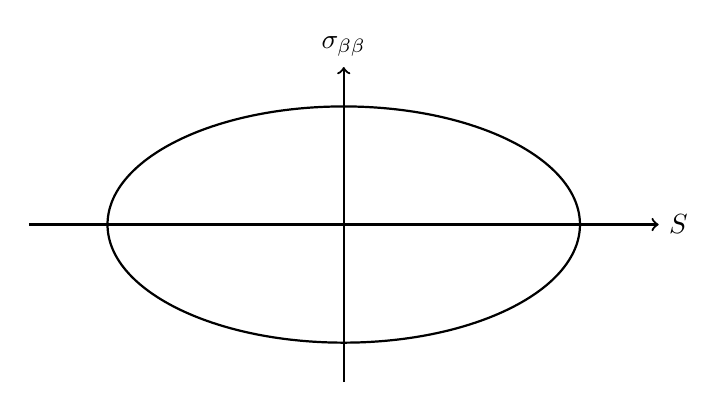
\begin{tikzpicture}
        \draw[thick] (0,0) ellipse (3 and 1.5);
        \draw[->,thick] (-4,0) -- (4,0) node[right] {\(S\)};
        \draw[->,thick] (0,-2) -- (0,2) node[above] {\(\sigma_{\beta\beta}\)};
    \end{tikzpicture}
    \caption{Elliptical window under internal pressure showing stress distribution directions.}
    \label{fig:elliptical_window}
\end{figure}

\subsection{Tangential Stress Distribution}
Using Eq. (2), the tangential stress distribution is computed and plotted around the elliptical window rim. Results are compared with material yield stresses.

\section{Computational Analysis}
\subsection{Model Setup}
The computational model consists of a large square plate containing three circular holes arranged in an equilateral triangle. Far-field traction \(S = 150 \, \text{MPa}\) is applied.

\begin{figure}[H]
    \centering
    \includegraphics[width=0.7\textwidth]{triangle_holes_model.pdf} % Replace with actual figure filename
    \caption{Geometric setup of three circular holes in a plate subjected to far-field traction.}
    \label{fig:three_holes}
\end{figure}

\subsection{Simulation Results}
Graphs of \(K_t\) variation with hole spacing (\(r/d\)) and load angle (\(\theta\)) are presented. Contour plots illustrate stress distributions for various plate sizes.

\begin{figure}[H]
    \centering
    \includegraphics[width=0.8\textwidth]{stress_contour_plot.pdf} % Replace with actual figure filename
    \caption{Stress contour plot for plate with three circular holes.}
    \label{fig:stress_contour}
\end{figure}

\section{Results and Discussion}
\subsection{Key Findings}
Theoretical and computational results highlight significant stress concentration near geometric discontinuities. The stress concentration factor increases as the plate size reduces or the hole spacing decreases.

\subsection{Implications}
Findings emphasize the need for careful material selection and structural reinforcement near high-stress regions in engineering designs.

\section{Conclusion}
This report demonstrates the critical role of stress concentrations in structural integrity. Theoretical and computational analyses provide valuable insights into stress distributions and their implications for design.

\newpage
\section*{References}
\begin{itemize}
    \item Timoshenko, S., and Goodier, J. N. \textit{Theory of Elasticity}, 3rd Edition. McGraw-Hill, 1970.
    \item Concept Analyst Tutorial, Durham University, 2025.
\end{itemize}

\section*{Appendices}
\subsection*{Appendix A: Parameters}
Detailed fuselage and plate parameters.

\subsection*{Appendix B: Concept Analyst Tutorial}
Step-by-step instructions for creating models and analyzing stress concentrations.

\end{document}
